En un local de lavado de autos ``CarLimpio'' se lava un auto a al vez, lo cual produce una cola de autos esperando ser atendidos.
La tasa de tiempo entre llegadas de autos a la cola es de 10 minutos, donde la llegada de un auto es independiente de la llegada de otro.
% Poisson
% llega 1/10 auto/min, = 0.1 auto/min = 6 auto/hora
\begin{itemize}
	\item ?`Cu\'al es la esperanza y varianza de llegada de autos a la cola por hora?\\
		$Esperanza\ =\ E(x)\ =\ \lambda\ =\ 6$\\
		$Varianza\ =\ V(x)\ =\ \lambda\ =\ 6$\\
	\item ?`Cu\'al es la probabilidad de que lleguen 5 autos en una hora?\\
		$P(X=5)\ =\ 0.1606231\ $\\ % dpois(5,6)
	\item ?`Cu\'al es la probabilidad de que lleguen mas de 7 autos en una hora?\\
		$P(X>7)\ =\ 1\ -\ P(X<=7)\ =\ 1\ -\ 0.7439798\ =\ 0.2560202\ $\\ %1 - ppois(7,6)
	\item Realice gr\'aficos de la funci\'on de densidad de probabilidad y de la funci\'on de distribuci\'on.\\
		%x<-seq(1,40) ; supongo que se le pueden dar cualquier valor, total hay que ver como se comporta...de 1 a 40 pienso que esta bien
		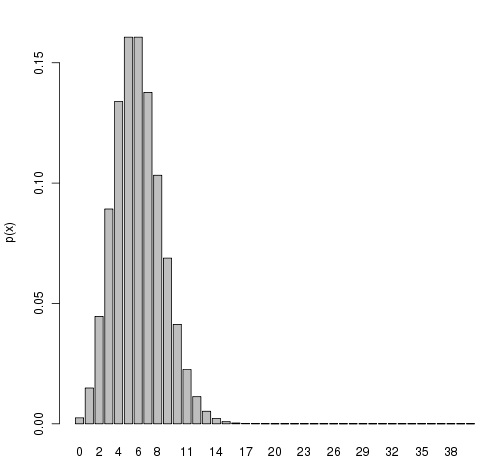
\includegraphics[scale=0.5]{images/1_4-dpois} \\%barplot(dpois(x,6),names.arg=x) 
		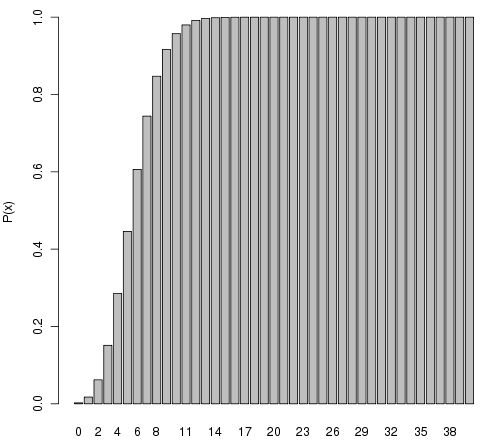
\includegraphics[scale=0.5]{images/1_4-ppois} \\%barplot(ppois(x,6),names.arg=x)
	\item Var\'ie el o los valores de los par\'ametros de la distribuci\'on y comente lo observado en los gr\'aficos de la funci\'on de densidad y de distribucii\'on. (2 casos)\\

	Caso 1: Variando el $\lambda$ a $20$:\\
	Funci\'on de densidad de probabilidad con $\lambda\ =\ 20$\\
  	  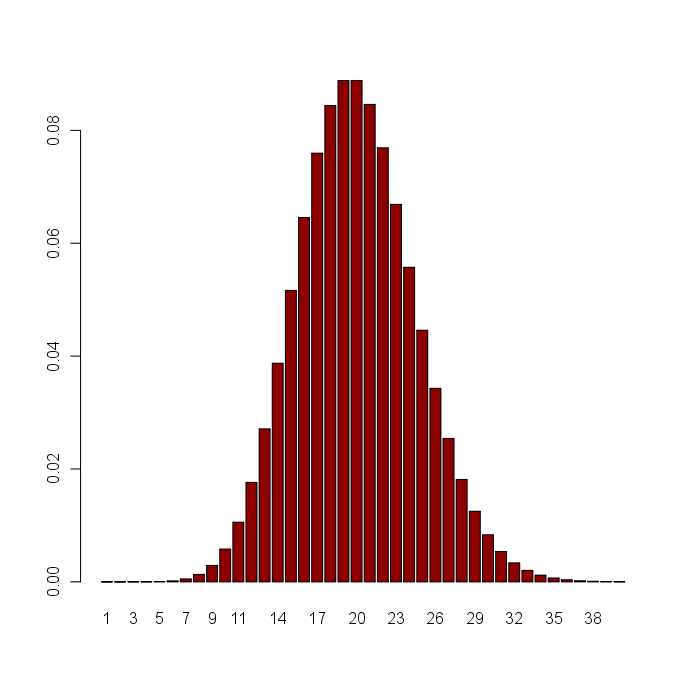
\includegraphics[width=3.3in,height=3.3in]{images/1_4-dpois20.png}\\
	Funci\'on de distribucion con $\lambda\ =\ 20$\\
  	  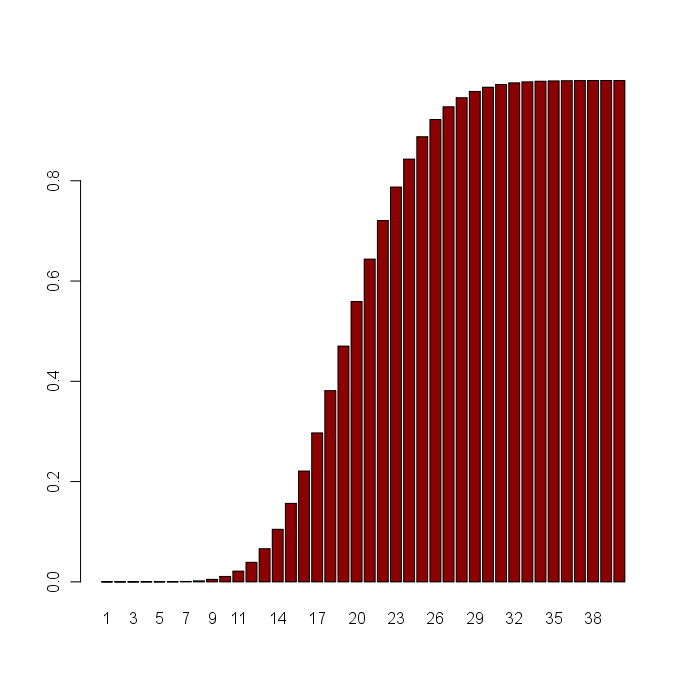
\includegraphics[width=3.3in,height=3.3in]{images/1_4-ppois20.png}\\
	Caso 2: Variando el $\lambda$ a $40$:\\
	Funci\'on de densidad de probabilidad con $\lambda\ =\ 40$\\
  	  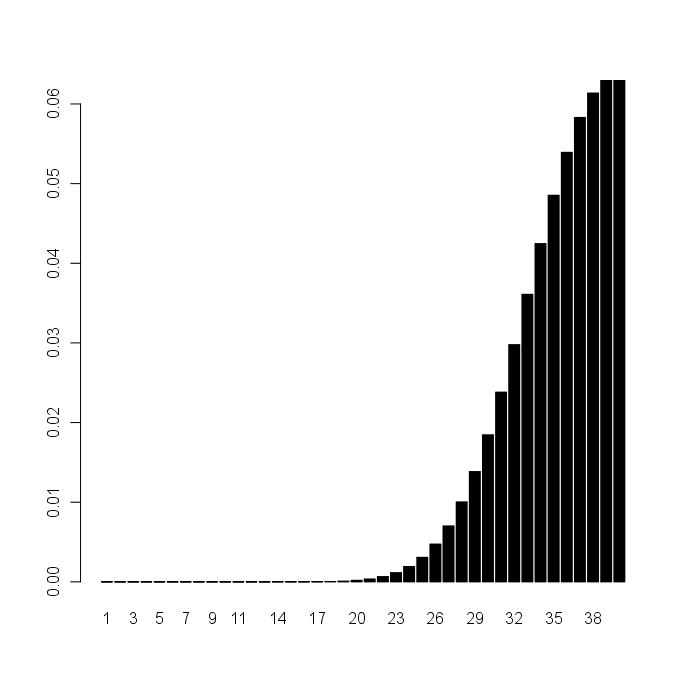
\includegraphics[width=3.3in,height=3.3in]{images/1_4-dpois40.png}\\
	Funci\'on de distribucion con $\lambda\ =\ 40$\\
  	  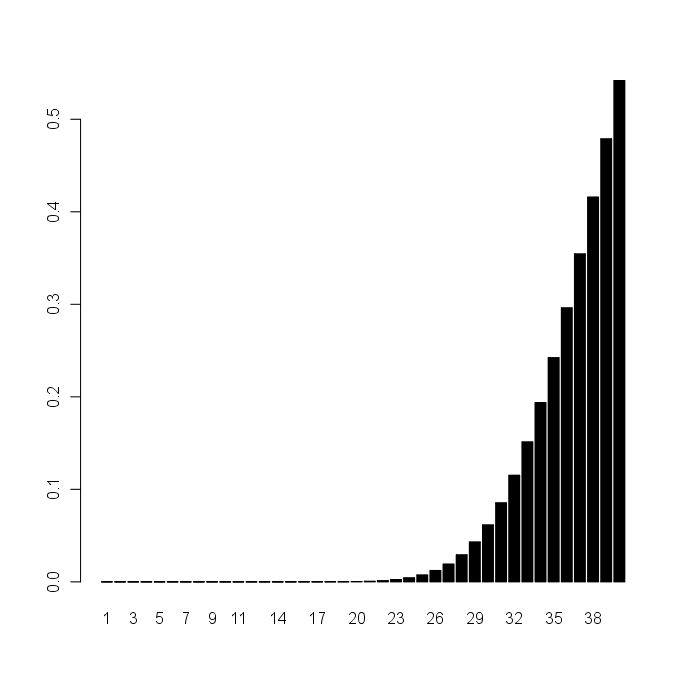
\includegraphics[width=3.3in,height=3.3in]{images/1_4-ppois40.png}\\

	Claramente podemos observar como al aumentar el parametro $\lambda$, la funcion de densidad y distribucion tiende a desplazarse hacia la derecha y ir disminuyendo la probabilidad maxima alcanzada.

\end{itemize}
